\documentclass{aa}
\usepackage{graphicx}
\usepackage{booktabs}
\usepackage{txfonts}
\usepackage{xcolor}
\definecolor{linkblue}{RGB}{25,70,110}
\usepackage[colorlinks=true,allcolors=linkblue]{hyperref}
\graphicspath{{figures/}}
\newcommand{\px}{\,\mathrm{px}}

\begin{document}
\title{Dating wide-field images of the night sky with planetary ephemerides}
\author{P. Thejll\inst{1}\corrauth{pth@dmi.dk}}
\institute{Danish Meteorological Institute, Skt. Kjelds Plads 11,
  DK-2100 Copenhagen~\O, Denmark}
\date{Received 13 September 2026 / Accepted ---}

\abstract
{Astronomical image metadata can be absent, altered, or less precise than the
celestial information recorded in the image itself. Wide-field photographs
often contain several planets whose changing relative positions provide an
independent calendar and clock.}
{We test whether a single circular-fisheye photograph can be dated by combining
a stellar astrometric solution with a blind search of planetary ephemerides.}
{Point sources were associated with Tycho-2 stars and fitted with the
eight-parameter Barghini fisheye model. Unmatched bright detections were
compared with topocentric positions of the planets from Mercury to Neptune on
a daily grid from 1950 through 2026. After selecting the best day from two
distinct planet--source associations, all image detections were reconsidered
and the epoch was refined continuously with three planets.}
{For a published image by F. Espenak, the blind daily search uniquely selected
2018 April 15. Mars, Jupiter, and Saturn were recovered independently, with
measured--predicted separations of 0.064, 0.213, and 0.352 pixels at the stated
time. The continuous three-planet minimum was 2018 April 15 07:08:16 UTC,
13 min 17 s after the published 06:55 UTC time. The stellar fit used 1213
associations and had 0.576-pixel RMS residual.}
{Planetary configurations can recover the date of a wide-field sky image and
can provide a sub-day timing constraint. In this first example the 13-minute
agreement is a best-fit offset, not a demonstrated timing precision: empirical
astrometric perturbations move the minimum by several hours. A joint treatment
of camera geometry, refraction, site, exposure interval, and ephemerides is the
natural route to defensible uncertainties.}
\keywords{astrometry -- methods: data analysis -- techniques: image processing
-- planets and satellites: detection -- atmospheric effects}
\maketitle

\section{Introduction}
\label{sec:introduction}

A sky photograph contains several kinds of time information even when its
header does not. Stellar proper motions encode long intervals, sidereal
rotation and star-trail lengths encode hours and exposure duration, and the
Moon and planets move against the stellar background on timescales from hours
to years. The planetary pattern is especially useful because it combines slow
changes in relative configuration, which identify a date, with faster apparent
motion and topocentric effects, which can constrain the time within that date.

Blind astrometric methods can identify the stellar coordinate system without
reliable image metadata \citep{Lang2010}. Circular-fisheye imagery adds a
strong, non-polynomial radial distortion and often reaches the horizon. Global
all-sky camera models have therefore been developed for meteor and night-sky
work \citep{borovicka1995,Barghini2019,Jeanne2019}. Once such a model maps every
detection onto the celestial sphere, ephemeris matching becomes an astronomical
dating problem rather than a visual identification exercise.

We demonstrate this idea on a public 180-degree image by Fred Espenak. Its web
page supplies a date, time, site, camera, and lens \citep{Espenak2018}, allowing
an external test of the inferred epoch. These labels were used for evaluation
and the final topocentric calculation; the published date and the named planets
were not supplied to the initial daily search. Section~\ref{sec:data} describes
the image, Sect.~\ref{sec:method} gives the astrometric and ephemeris procedure,
and Sect.~\ref{sec:results} compares the recovered solution with the published
metadata. We end with the attainable information and the remaining limitations.

\section{Image and catalogue data}
\label{sec:data}

The test image is \emph{Southern Milky Way and Planets}, photographed at
Atacama Lodge near San Pedro de Atacama, Chile. The publisher states 2018 April
15 at 06:55 UTC, a Nikon D750, a Sigma 8-mm circular fisheye, and one 240-s
exposure at $f/4.5$ and ISO 1600 \citep{Espenak2018}. The published original is
$4016\times4016$ pixels; we analysed the available $925\times925$-pixel JPEG.
The file metadata likewise report a Nikon D750, 8.0-mm focal length, 240 s,
$f/4.5$, and ISO 1600. Its lens-model field instead gives 8.0 mm at $f/3.5$;
we retain this discrepancy as metadata rather than using either lens label as a
fit constraint.

We used a fixed local copy of the Tycho-2 catalogue \citep{Hog2000}, augmented
by bright Hipparcos stars where required. Catalogue coordinates with two
proper-motion components were propagated to the candidate epoch. A scan of the
stellar residual against catalogue reference year was also made as a check on
whether proper motion alone dated this recent image.

\begin{figure*}
  \centering
  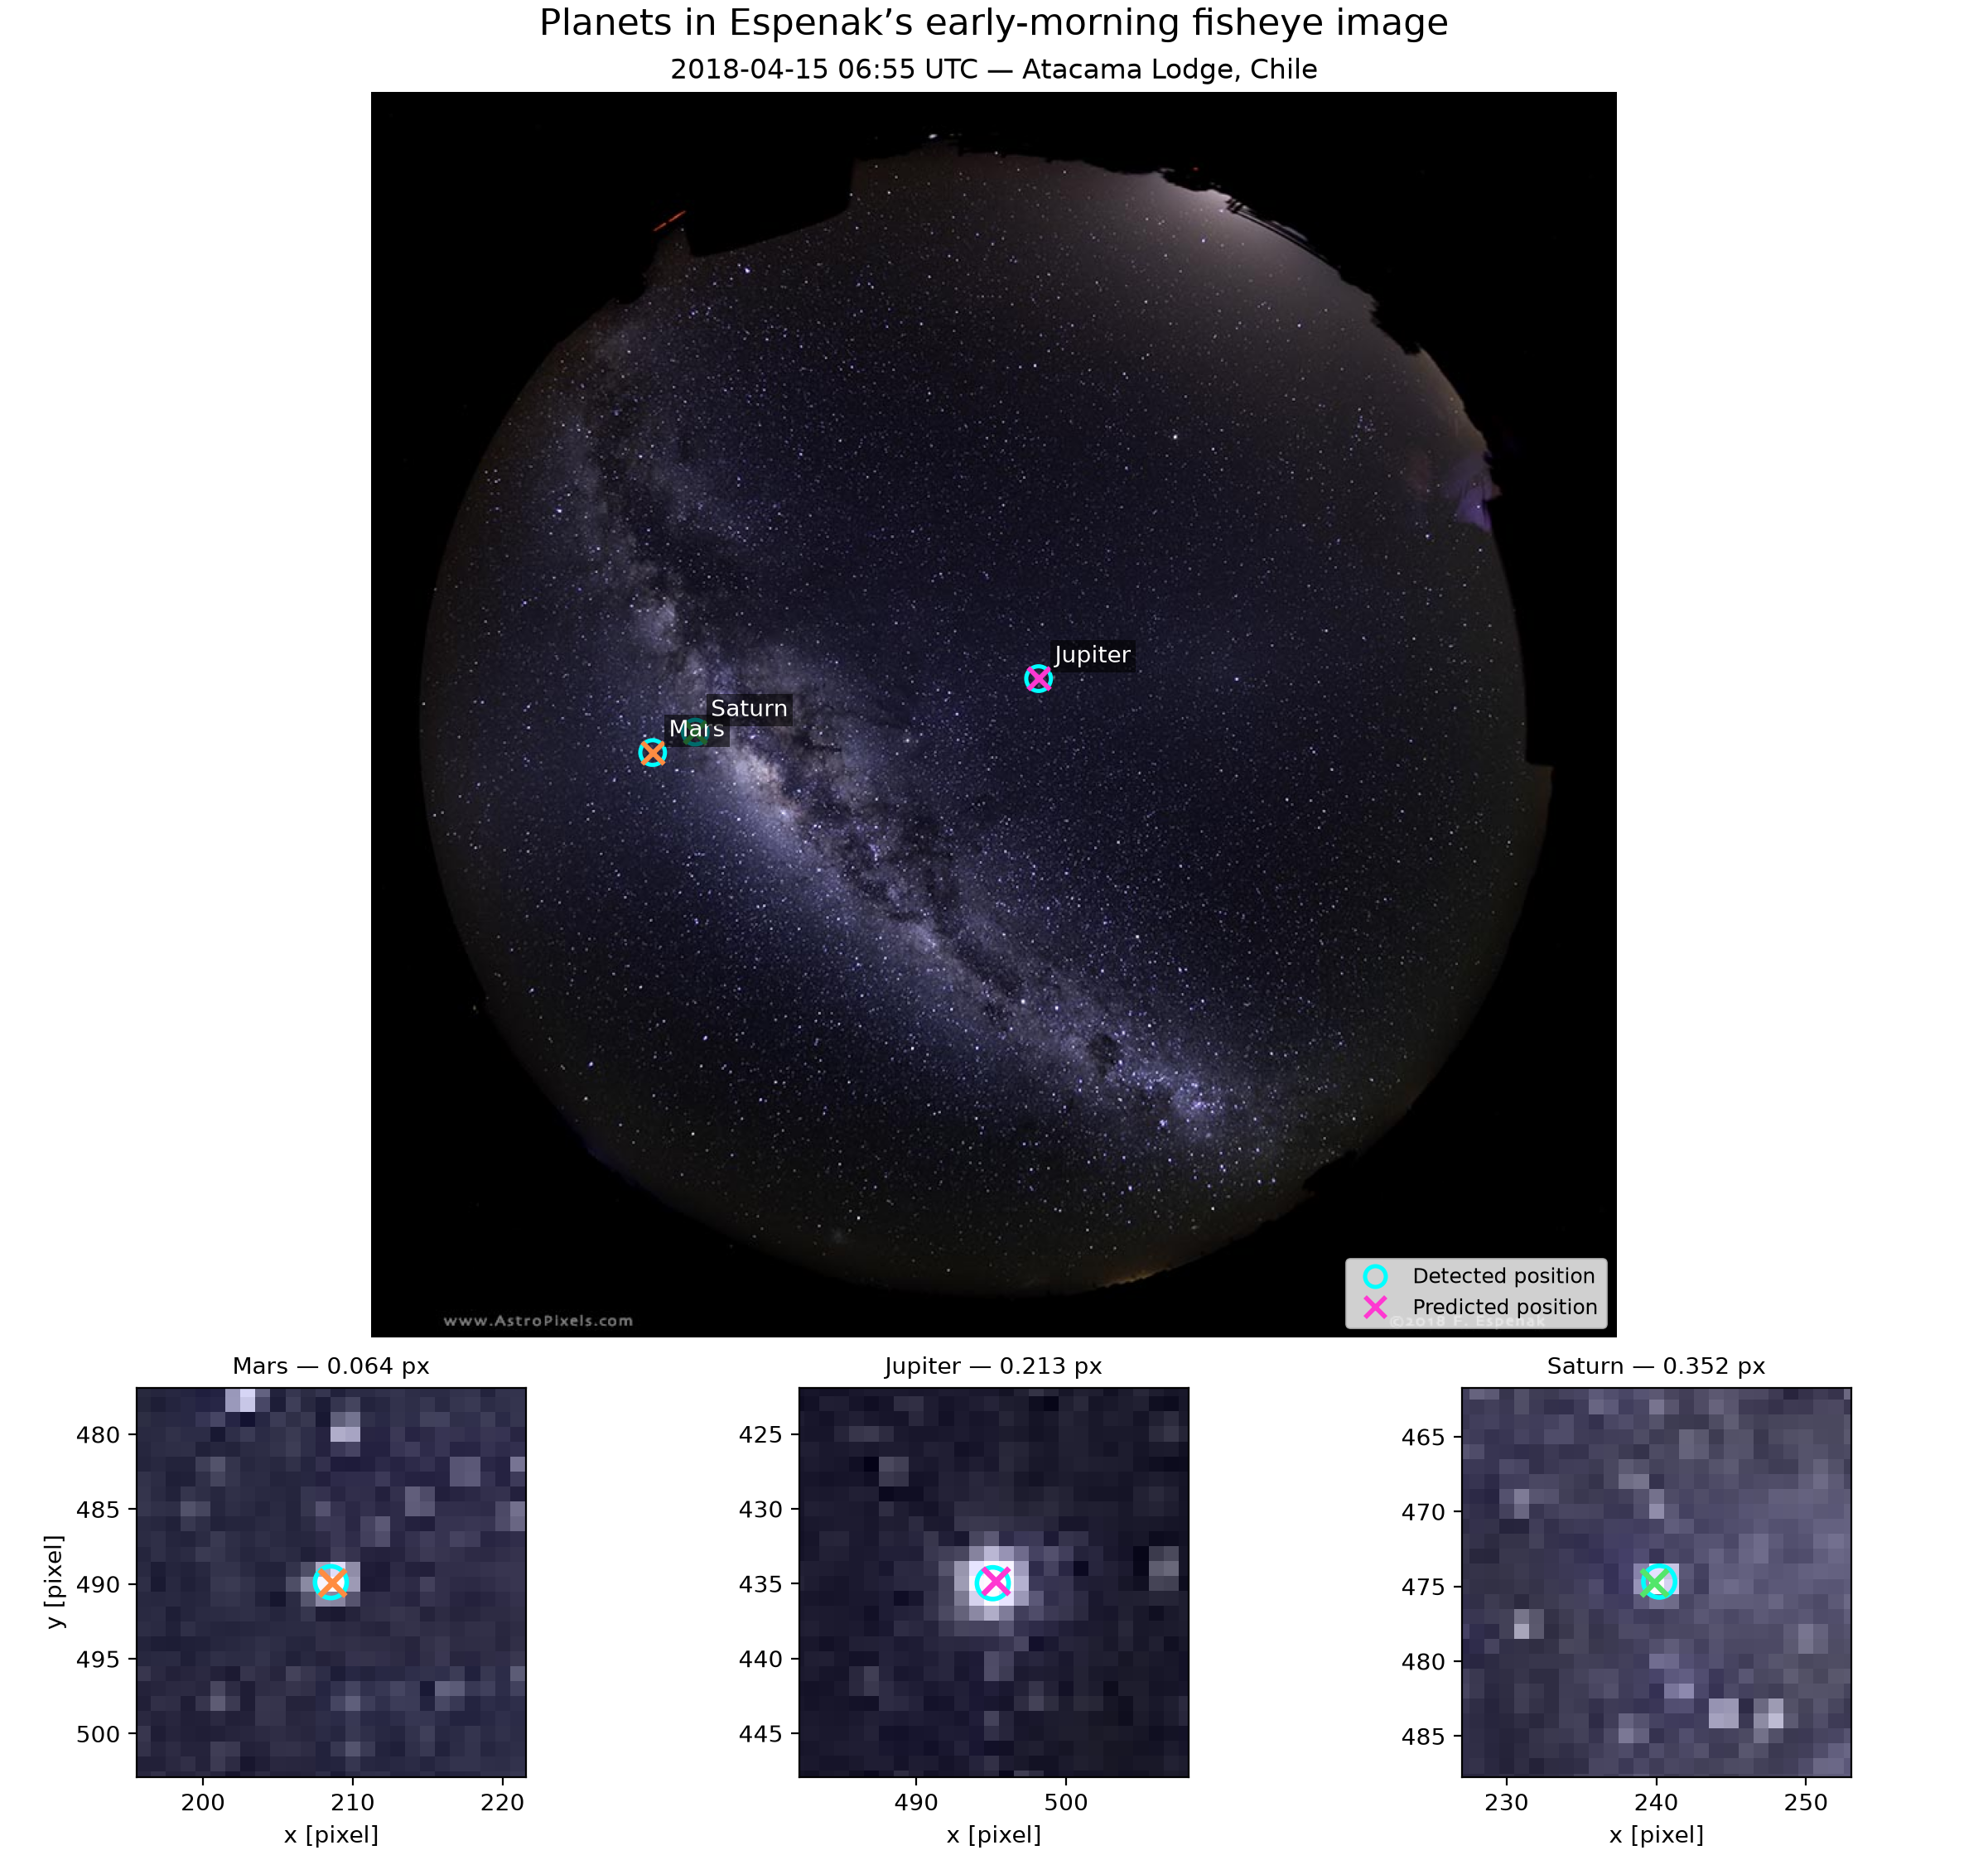
\includegraphics[width=0.88\textwidth]{planet_measured_vs_predicted_overlay.png}
  \caption{Espenak's fisheye image with the three recovered planets. Cyan
  circles show the measured source centroids; coloured crosses show the
  topocentric ephemeris positions projected through the fitted camera model at
  the published epoch. The lower panels show the same coordinates at native
  pixel scale.}
  \label{fig:overlay}
\end{figure*}

\section{Method}
\label{sec:method}

\subsection{Source association and global camera model}

Point sources were detected after local background subtraction. Growing
measurement windows retained broad and saturated sources. We obtained a small
initial constellation with \texttt{tetra3}, ESA's open-source Python
astrometric plate solver for star trackers \citep{tetra3}. Its
``lost-in-space'' pattern matching identifies stars and determines the camera
pointing in right ascension and declination without an initial pointing
estimate. It therefore removes the need for a user-supplied initial sky
pointing or WCS in our workflow, while its solution initialises the subsequent
Barghini-model fit. This does not remove all prior information: tetra3 requires
an approximate field-of-view range and a compatible pattern database. Its
distributed default database covers fields of view from $10^\circ$ to
$30^\circ$ and stars down to magnitude~7 \citep{tetra3}.

Progressive nearest-neighbour association then expanded the solution over the
complete circular field. Every detected source remained available for
association. No catalogue identifier or saved solution was used to seed this
demonstration.

The global projection is the eight-parameter model of
\citet{Barghini2019}, expressed with independent detector positions for the
optical centre $O=(x_O,y_O)$ and reference direction $Z=(x_Z,y_Z)$. For a
detector radius $r_O$ about $O$, the projection angle $u$ is
\begin{equation}
  u(r_O)=V r_O+S\left[\exp(D r_O)-1\right].
  \label{eq:radial}
\end{equation}
The remaining parameter $a_0$ fixes the azimuthal orientation. The transformation
from $(u,b)$ about the optical axis to a celestial unit vector follows the
spherical rotation in Eqs.~(5), (6), and (11) of \citet{Barghini2019}. We fit
the eight parameters by minimising detector-plane residuals between measured
centroids and catalogue directions projected into the image. In the present
celestial solution $Z$ is a fixed bootstrap reference direction; it should not
be interpreted as a fitted terrestrial zenith.

The catalogue-to-camera fit is independent of the manufacturer's nominal
fisheye projection. Its radial mapping, optical centre, and orientation are
therefore inferred from stars. Refraction was not included in this first
planetary experiment. This omission is most consequential near the horizon and
is carried into the empirical residuals rather than corrected cosmetically.

\subsection{Blind date search and continuous refinement}

The image positions of all detections were inverted through the fitted camera
model to celestial unit vectors. We evaluated topocentric apparent positions
of Mercury, Venus, Mars, Jupiter, Saturn, Uranus, and Neptune using Astropy's
solar-system transformations \citep{Astropy2022}, whose built-in planetary
model is based on the conventional analytical elements of \citet{Simon1994}.
The stated observing site was used for this topocentric step; geographical
position was not fitted in the experiment reported here.

For every day from 1950 January 1 through 2026 December 31, we found the best
assignment of two different planets to two different initially unmatched
sources and recorded
\begin{equation}
  Q_2(t)=\left[\frac{1}{2}\sum_{p=1}^{2}
       \Delta\theta_p(t)^2\right]^{1/2},
  \label{eq:q2}
\end{equation}
where $\Delta\theta_p$ is the great-circle distance between a measured source
and a planet. Restricting the blind stage to distinct source--planet pairs
prevents a single bright object from satisfying both assignments. At the best
day we again searched \emph{all} detections, rather than preserving the
unmatched classification, and accepted unique associations within
$0.25^\circ$. This recovered a third planet. Holding those three associations
fixed, we minimised the analogous three-planet RMS $Q_3(t)$ continuously within
$\pm2$ d of the daily solution.

This staged procedure separates discovery from precision. The daily search
asks whether the planetary configuration supplies a distinctive calendar date;
the continuous fit measures where the astrometric residual is smallest on that
date. To probe sensitivity to camera-model errors, we drew 2000 sets of three
two-dimensional residual vectors from the fitted stellar residuals, added them
to the planetary centroids, and repeated the fine timing search. This is an
empirical perturbation test, not a formal confidence interval: it neglects
correlated distortion, catalogue systematics, refraction, and uncertainty in
the site.

\section{Results}
\label{sec:results}

\subsection{Stellar and lens solution}

The image yielded 1255 detections, of which 1213 were associated with catalogue
stars; 42 remained unmatched and none was withheld. The camera fit has an RMS
residual of $0.576\px$, a median of $0.367\px$, and a 90th percentile of
$0.745\px$. The fitted optical centre is $(463.79,460.84)\px$. The radial
coefficients are $V=0.00310691$ rad px$^{-1}$, $S=0.00710973$ rad, and
$D=0.00764440$ px$^{-1}$. The implied $90^\circ$ radius is $441.17\px$, and
the central derivative of Eq.~(\ref{eq:radial}) is
$0.18113^\circ$ px$^{-1}$.

At the original $4016$-pixel sampling, the fitted horizon radius would be about
1915 pixels under uniform rescaling, giving a 3830-pixel image circle. This is
consistent with a circular fisheye nearly filling Espenak's square frame. The
agreement is a physical cross-check on the published Nikon D750 and 8-mm Sigma
description; the fit itself used neither camera nor lens metadata. The left
panel of Fig.~\ref{fig:lensdate} also shows that the fitted mapping is not
exactly equidistant, illustrating why the catalogue-derived lens model is
needed for the planetary comparison.

\begin{figure*}
  \centering
  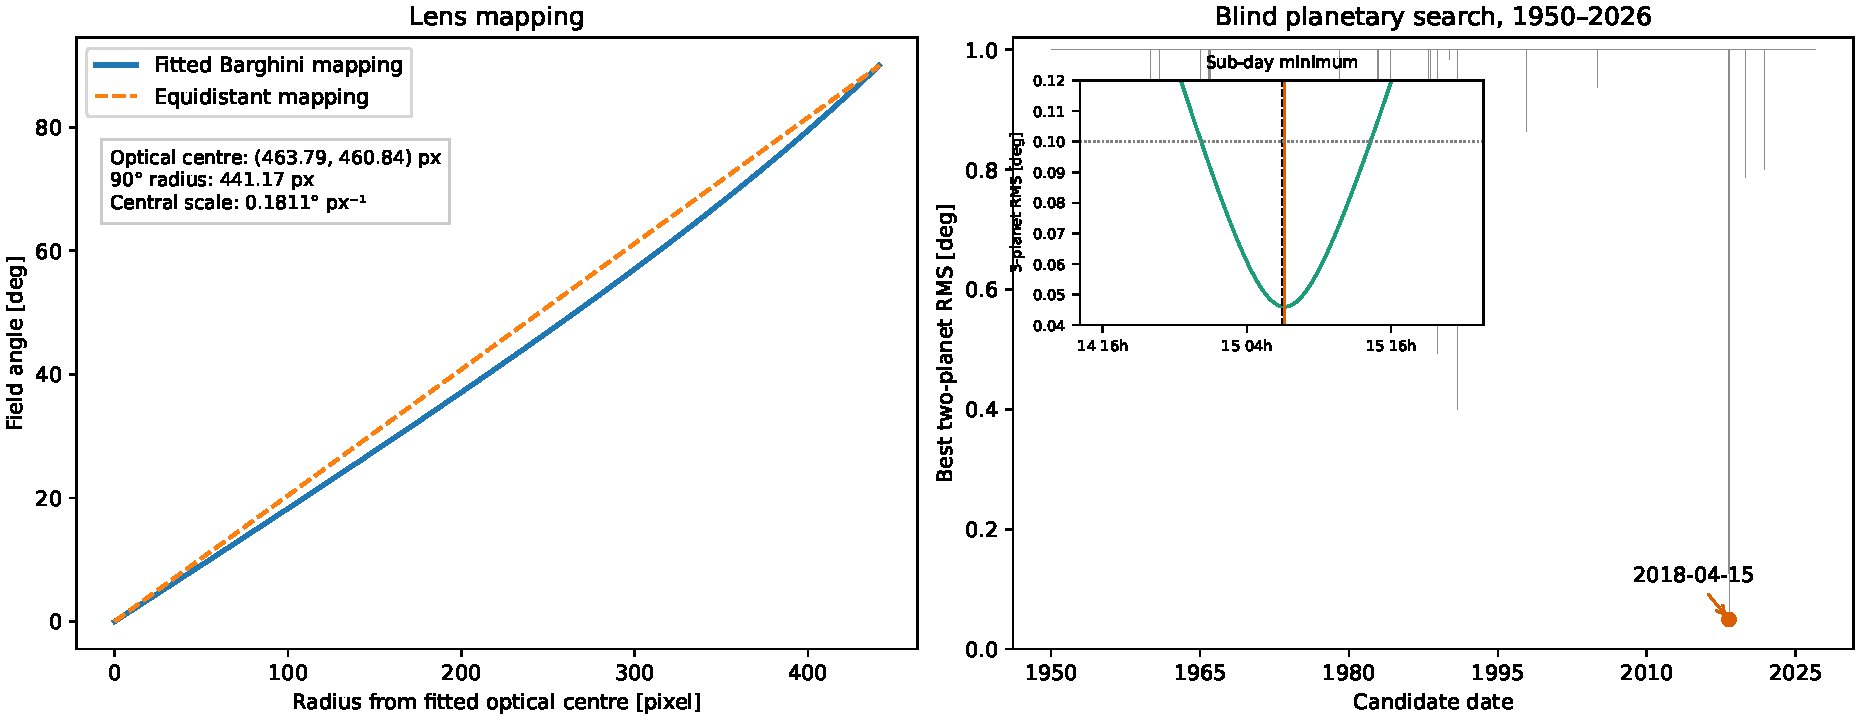
\includegraphics[width=\textwidth]{lens_and_epoch_solution.pdf}
  \caption{Left: fitted Barghini radial mapping and an equidistant mapping with
  the same $90^\circ$ radius. Right: the blind two-planet objective over
  1950--2026, clipped at $1^\circ$ for display. The inset gives the continuous
  three-planet objective around the selected date; dashed and orange vertical
  lines mark the published and best-fitting epochs, respectively.}
  \label{fig:lensdate}
\end{figure*}

\subsection{Planetary date and time}

The blind daily minimum occurred on 2018 April 15, the published date. Its
Jupiter and Saturn assignments had a two-planet RMS of $0.0494^\circ$. After
suppressing dates within 45 d of this solution, the next minimum was 1990
December 19 with $0.4002^\circ$ RMS, eight times larger. Only 18 daily trials
over the 77-year interval fell below $0.5^\circ$, so the global minimum is
strongly distinguished.

Reconsidering all sources on the selected date independently recovered Mars,
Jupiter, and Saturn as detections 36, 8, and 54. At the stated time their
detector-plane residuals were 0.064, 0.213, and 0.352 pixels, respectively
(Fig.~\ref{fig:overlay} and Table~\ref{tab:planets}). The other searched planets
were below the local horizon. The fixed-association continuous minimum was
2018 April 15 07:08:16 UTC with $Q_3=0.0460^\circ$, an offset of 13 min 17 s
from the stated 06:55 UTC.

\begin{table}
  \caption{Recovered planets at the published epoch.}
  \label{tab:planets}
  \centering
  \begin{tabular}{lrr}
    \hline\hline
    Planet & Detection & Separation [pixel] \\
    \hline
    Mars    & 36 & 0.064 \\
    Jupiter &  8 & 0.213 \\
    Saturn  & 54 & 0.352 \\
    \hline
  \end{tabular}
\end{table}

The small offset is an accuracy check against external metadata, rather than a
$13$-minute uncertainty. The interval over which $Q_3<0.1^\circ$ is about
14 h. In the empirical residual-vector experiment, the 16th, median, and 84th
percentiles of the fitted-time displacement were $-2.92$, $-0.08$, and
$+3.00$ h. The 240-s exposure introduces a further two-minute convention shift
if the published time refers to an endpoint rather than mid-exposure. Proper
motion did not usefully constrain this recent date: among the 1127 matched stars
with both components, a reference-year scan changed the RMS by only
$9.8\times10^{-6}\px$ between 2009 and 2018.

\section{Perspectives}
\label{sec:perspectives}

Dating a single sky image to the correct day is useful wherever provenance is
incomplete: digitised plate and film collections, meteor and auroral archives,
environmental all-sky cameras, and historical or public astrophotography. Large
photographic archives already open century-long time baselines
\citep{Grindlay2009}; an astronomical timestamp can expose catalogue mistakes,
order undated sequences, and connect an image to observing logs or transient
events. In particular, a date recovered for a historical image containing a
nova could place that observation on the nova light curve and constrain its
rise, peak, or decline. This is valuable for epochs before systematic patrol
cameras supplied dense time-series coverage. A planetary solution is also
independent of file timestamps and many camera-clock failures.

The 13-minute agreement in this example is interesting because it comes from
the celestial scene in one static exposure, but it should be understood as a
target for a coupled model. Planetary angular velocities near the observed
configuration convert small astrometric biases into hours of timing shift. A
fit that simultaneously includes a physical zenith, latitude, atmospheric
refraction and extinction, camera geometry, and the finite exposure should
separate these effects. Star-trail angular length can supply exposure duration;
the distribution of photometric residual against airmass can constrain the
zenith and extinction; and the resulting terrestrial orientation can supply
local sidereal time. Together these observables could turn the sharp formal
planetary minimum into a defensible sub-hour uncertainty and might constrain an
unknown observing latitude as well as the epoch. Testing that prospect requires
multiple images, deliberately blinded metadata, and injected perturbations.

\section{Conclusions}

A global stellar astrometric solution and a blind planetary ephemeris search
recovered the published date of a 180-degree fisheye photograph over a
1950--2026 search interval. Three independently recovered planets placed the
continuous minimum 13 min 17 s from the stated time, while their predicted
positions agreed with the measured centroids to better than 0.36 pixel. The
catalogue-fitted Barghini mapping was consistent with the published circular
8-mm fisheye geometry and avoided assuming an ideal manufacturer projection.

The experiment establishes calendar recovery and close agreement with an
external timestamp. Its present several-hour empirical sensitivity shows where
the scientific work now lies: coupled refraction, orientation, site, exposure,
and camera modelling, followed by validation on a blinded image set.

\begin{acknowledgements}
We thank Fred Espenak for publishing the image and its observing metadata. The
image remains credited to and copyrighted by its photographer; its use here is
for scientific analysis. This work made use of Astropy and tetra3.
\end{acknowledgements}

\section*{Data and code availability}
The figure-generation code, numerical summary, and verification tests accompany
this manuscript repository. The complete analysis code, fitted parameters,
source associations, and machine-readable planetary matches will be deposited
as a versioned Zenodo record upon acceptance; the final DOI will replace this
statement. The input photograph is available from the publisher's linked image
page, subject to the photographer's terms \citep{Espenak2018}.

% BODY

\bibliographystyle{aa}
\bibliography{references}
\end{document}
